\documentclass[12pt]{article}
\usepackage[english]{babel}
\usepackage[utf8]{inputenc}
\usepackage{color}
\usepackage[a4paper,lmargin={2cm},rmargin={2cm}, tmargin={2cm},bmargin = {2cm}]{geometry}
\usepackage{amssymb}
\usepackage{amsmath}
\usepackage{mathtools}
\usepackage{graphicx}
\usepackage{cite}
\usepackage{wallpaper}
\usepackage{amstext}
\usepackage{blindtext}
\usepackage{multicol}
\usepackage[singlespacing]{setspace}
\usepackage{tabulary}
\usepackage{tabularx}
\usepackage[T1]{fontenc}
\usepackage{float}
\usepackage{csquotes}
\usepackage{todonotes}

\usepackage{placeins}
\usepackage{afterpage}

\renewcommand{\labelitemi}{$\bullet$}
\renewcommand{\labelitemii}{$\cdot$}
\renewcommand{\labelitemiii}{$\circ$}
\renewcommand{\labelitemiv}{$\ast$}

\usepackage{caption}
\usepackage{framed}
\definecolor{shadecolor}{rgb}{0.6,0.6,0.61}

%\bibliographystyle{alphadin}
\bibliographystyle{IEEEtran}

\begin{document}
%\hyphenation{Ver-schlüsselungs-verfahren}

\begin{titlepage}
\ThisCenterWallPaper{1.0}{h-logo-background}	

%  \HoleMask

%  \hspace{-3cm}
  \begin{minipage}[t]{10cm}
  %\vspace{2cm}
  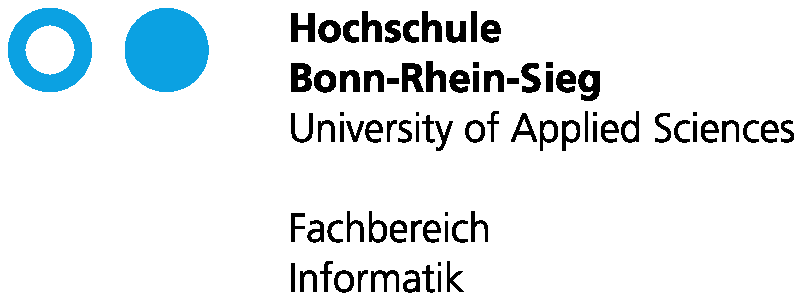
\includegraphics[width=10cm]{h-logo-full-font-embed}\\
  \end{minipage}
  \vspace{2.5cm}

	\begin{center}

    \vspace{0.8cm}

    \vspace{3cm}
    \begin{Huge}
    \textbf{Exposé}\end{Huge}\\
    \vspace{0.8cm}
  	\begin{huge}
  	\textbf{TITEL}
  	\end{huge}
  	 \vspace{0.6cm} \\
  	  	  \begin{large}von
  	  \end{large}
  	  \\ \begin{LARGE}
  	   \vspace{0.6cm}
  	  {Jan Kruska}\\
  	  9028385\\
  	  \vspace{0.8cm}
  	 
  	\end{LARGE}
  	
    \vspace{3.0cm}
			\end{center}
	\begin{large}
%	\begin{flalign}
%	\hspace{4.5cm} 
	%\text{Referee and Tutor:} \hspace{1.2cm}		&\text{Prof. Dr. Alexander Asteroth}& % \notag\\&31.12.2016  \notag
%\end{flalign} 

\begin{table}[h!]
\begin{tabularx}{\textwidth}{l@{\hspace{2.0cm}}X}

Betreut durch: & Prof. Dr. Alexander Asteroth\\
und: &  Alexander Hagg, M.Sc.\\



\end{tabularx}
\end{table}  
  
\end{large}
%  \vspace{0.5cm}
%  \vfill
\end{titlepage}


\pagenumbering{arabic}
\tableofcontents
\newpage{}


\section{Einleitung}

Die Domäne der Aerodynamik stellt durch ihre Komplexität sowohl für Mensch als auch Computer eine große Herausforderung dar.
Die physikalischen Gesetze denen diese folgt sind zwar bekannt, deren Zusammenspiel allerdings so stark ineinander verwoben, das beim Design aerodynamischer Körper oft auf Faustregeln zurückgefallen werden muss.
Durch computergestützte Assistenz könnte dieser Designprozess erheblich verbessert werden.

Evolutionäre Taktiken haben sich in der Vergangenheit als mächtige Heuristik zur Untersuchung komplexer Problemräume bewiesen.
Die Untersuchung inwieweit solche Taktiken für die Nutzung in der computergestützten Assistenz nützlich sind liegt nahe.
Eine Methode die sowohl in der Lage ist neben Lösungen auch Wissen über den Lösungsraum zu generieren könnte den Designprozess erheblich vereinfachen indem sowohl Initiallösungen, von denen eine weitere menschliche Optimierung ausgehen kann, als auch Wissen über das Problem, womit diese weitere Optimierung zielstrebiger erfolgen kann, erzeugt werden.



\section{Problembeschreibung}

\subsection{Radkastendomäne}

\subsection{E-Roller-Domäne}

Genetische Algorithmen sind eine effektive  Methode um "kreative" Lösungen für komplexe Probleme zu generieren.
Allerdings haben viele evolutionäre Algorithmen die Tendenz, das gefundene Lösungen im Verlauf der Algorithmen immer mehr zu einer Lösungsklasse konvergieren.
Das Ergebnis sind damit am Ende $n$ minimal unterschiedliche Variationen der selben Lösung.
Dies führt zu zwei Hauptproblemen. Erstens neigen solche Algorithmen dazu in lokalen Optima "stecken" zu bleiben, da das Verlassen eines lokalen Optimums immer mit einer Fitnesseinbuße verbunden ist.
Zweitens produzieren solche Algorithmen zwar eine Lösung, warum diese Lösung allerdings geeignet ist, ist für einen menschlichen Beobachter im Nachhinein nicht unbedingt ersichtlich.
Damit kann der menschliche Beobachter auch nicht einschätzen, ob die erhaltene Lösung tatsächlich die global beste Lösung ist, und wenn sie das nicht ist wie in Richtung des globalen Optimums weiteroptimiert werden kann.

Es wurden verschiedene Diversitäts Ansätze vorgeschlagen, die sich grundsätzlich in genotypische und phänotypische Diversitätsansätze unterscheiden lassen.
Ansätze die Diversität auf Genotyp-Ebene gewährleisten, tendieren dazu nur die erste Problematik, die definitiv auch die größere ist, zu adressieren.
Ansätze die Diversität im Phänotyp definieren sind hier wesentlich interessanter, da sie in der Lage sind Wissen über den tatsächlichen Lösungsraum zu erzeugen.
Diese Ansätze werden allgemein unter dem Begriff von Quality-Diversity- und Illuminations-Algorithmen zusammengefasst.
Diese liefern typischerweise eine Vielzahl an diversen möglichen Lösungen, durch die nicht selten das Problem und Zusammenhänge zwischen Lösungseigenschaften und Lösungsqualität besser verstanden werden kann.

 
\section{Literatur}

\subsection{MAP-Elites}
\label{sub:mapElites}
MAP-Elites \cite{Mouret.4202015} ist ein genetischer Algorithmus der phänotypische Diversität gewährleistet.
Dies geschieht durch eine Aufteilung des Lösungsraum entlang n Dimensionen, die Eigenschaften der Lösung darstellen.
Dadurch wird der Lösungsraum in phänotypische Zellen eingeteilt.
Jede dieser Zellen kann eine Lösung enthalten, die nur durch eine andere bessere Lösung, die in die gleiche Zelle passt ersetzt werden kann.
Neben einer Vielzahl von Lösungen kann diese Karte auch dabei helfen die Problemdomäne besser zu verstehen, indem Zusammenhänge zwischen den Kategorien, nach denen klassifiziert wurde und der Qualität der Lösungen, aufgedeckt werden.
\todo[inline]{umformulieren, umstrukturieren, Quelle}

\subsection{Surrogat-Modell}
\label{sub:surrogate}
Für die Selektion von Individuen innerhalb eines genetischen Algorithmus wird die Lösungsqualität dieser Individuen, typischerweise Fitness genannt, benötigt.
Außerdem findet die Auswertung der Fitnessfunktion innerhalb des genetischen Algorithmus sehr häufig statt.
Dies stellt bei relativ einfachen Fitnessfunktionen keine große Einschränkung dar, auf Problemdomänen in denen die Auswertung der Fitness eines Individuums allerdings komplexer und dadurch zeitaufwändiger wird, kann dies die Anwendbarkeit einfacher genetischer Algorithmen einschränken.

Aerodynamische Probleme, für die zeitaufwendige Simulationen nötig sind, gehören ohne Zweifel zu der Klasse von Problemen für die die Anzahl der benötigten Funktionsauswertungen zu groß sind, als das der Algorithmus in vertretbarer Laufzeit abschließen kann.
Um genetische Taktiken auf eine solche Problemdomäne anzuwenden, wird eine Möglichkeit benötigt die benötigten Funktionsauswertungen erheblich zu reduzieren.
Eine solche Möglichkeit ist ein Surrogatmodell \cite{Jin.2011}\cite{Preen.2016}, eine Machine-Learning Modell, welches aufgrund echter Simulationsauswertungen trainiert wird um deren Ergebnis annähernd vorherzusagen.
Eine Auswertung des Modells erfordert dabei nur einen winzigen Bruchteil des Aufwands der für eine Simulation nötig wäre.
Theoretisch sind verschiedenste Machine-Learning Verfahren für das Surrogatmodell denkbar, Gaußprozesse bieten sich durch die Eigenschaft an, dass sie neben einer Vorhersage auch immer ihre eigene Unsicherheit Liefern, und entsprechend Bereiche zeigen können in denen große Unsicherheit herrscht, sprich in denen der Gaußprozess wenig weiß.
Der Nachteil der hohen Komplexität von Gaußprozessen \todo[inline]{genaue Komplexität? Quelle: \cite{Rasmussen.2008}} ist durch die Limitierung auf eine geringe Anzahl an Simulationen, und damit der Limitierung auf einen kleinen Trainingsdatensatz vernachlässigbar.
\todo[inline]{Abschnitt erfolgreiche Anwendung von Surrogat-Modellen und genetischen Algorithmen, sth. about Orders of magnitude evaluation reduction}

\subsection{SAIL}

SAIL (Surrogate-Assisted Illumination) vereint die in \ref{sub:mapElites} und \ref{sub:surrogate} beschriebenen Ansätze.
In \cite{Gaier.6152018} wurde gezeigt, dass dieser Ansatz erfolgreich auf 2D und 3D aerodynamische Domänen angewandt werden kann.
\todo[inline]{Inwieweit sollen Anpassungen vorgenommen werden? Feature-Dimensionen,zusätzliche Contraints etc. }

\todo[inline]{Thesis von Sascha zwar nicht zitierfähig aber draufeingehen doch vermutlich sinnvoll}
\section{Ansatz}


\section{Leistungen}
Mindestergebnis:
\begin{itemize}  
\item Die Implementierung des produziert für die Radkastendomäne eine Karte aus semantisch korrekten Verformungen der Radkästen.
\item Die Implementierung liefert für die Radkastendomäne diverse Lösungen.
\todo[inline]{Arbeit enthält a,b,c}
\end{itemize}
Erwartetes Ergebnis:
\begin{itemize}  
\item  Die Implementierung liefert für die Radkastendomäne Lösungen die den Constraint erfüllen.
\end{itemize}
Maximalergebnis:
\begin{itemize}  
\item Die Implementierung liefert für die E-Roller-Domäne eine Karte aus diversen Lösungen
\item Die Implementierung liefert für die E-Roller-Domäne Lösungen die die Constraints erfüllen
\end{itemize}

\newpage{}

%\section{Literature}%

\begin{appendix}
\section{Struktur Thesis}

\begin{enumerate}
	\item Eidesstattliche Erklärung
	\item Abstract
	\item Grundlagen
	\begin{itemize}
		\item Genetische Algorithmen
		\item MAP-Elites
		\item Surrogat-Modell
		\item Probleme \& Herausforderungen von bestehenden Ansätzen \todo{Sascha?}
	\end{itemize}
\item Methode
\begin{itemize}
	\item Radkastendomäne
	\item E-Roller-Domäne
	\item Wahl der Features
	\item Design-Constraints und das daraus resultierende Design der Fitnessfunktion
\end{itemize}
\item Ergebnis Radkastendomäne
\begin{itemize}
	\item Experimente
	\item Analyse
	\item Zusammenfassung
\end{itemize}
\item Ergebnis E-Rollerdomäne
\begin{itemize}
	\item Experimente
	\item Analyse
	\item Zusammenfassung
\end{itemize}
\item Diskussion
\item Ausblick
\item Literaturverzeichnis
\item Anhang
\end{enumerate}

\section{Zeitplanung und Aufgaben}

\end{appendix}
  
\newpage{}
\section{Literaturverzeichnis}
\bibliography{expose,citavi}
\newpage{}

\end{document}}